\chapter[Electron Density Mapping in Carina Nebula]{Electron Density Mapping in Carina Nebula}
\label{ch:carina}

To map electron density in Carina we begin with the following equation from \cite{pineda2018}.
\begin{equation}
    R^{[NII]}_{RRL} = 2.68 \times 10 ^ {-9} \nu_{RRL} T_e^{3/2} \frac{f(^3\text{P}_1)}{n_e} G^{-1}_{NLTE}(n_e,T_c)X_N
    \label{eq:ratio}
\end{equation}
In this equation we have the following variables:
\begin{itemize}
    \item $R^{[NII]}_{RRL}$: The ratio of the intensity of NII to the intensity of the Hydrogen Radio Recombination Line (RRL).
    \item $\nu_{RRL}$: The frequency of the RRL in Hz.
    \item $T_e$: The electron temperature in Kelvin.
    \item $f(^3\text{P}_1)$: The fractional population of the $^3\text{P}_1$ level of ionized nitrogen. 
    \item $n_e$: The electron density in cm$^{-3}$.
    \item $G_{NLTE}(n_e,T_c)$: The deviation from local thermodynamical equilibrium (LTE) for the hydrogen RRL emission.
    \item $X_N$: The abundance of nitrogen with respect to hydrogen.
\end{itemize}

Both $T_e$ and $X_N$ can be estimated using the distance to the Galactic center $R_{gal}$ in kiloparsecs (kpc). 
\begin{align}
    T_e &= (4446 \pm 301) + (467 \pm 34) R_{gal} \\
    12 + log(X_N) &= (8.21 \pm 0.09) - (0.059 \pm 0.009) R_{gal}
\end{align}

To solve for $n_e$ we can isolate the terms that rely on $n_e$ in Equation (5.1).
\begin{equation}
    \frac{f(^3\text{P}_1)}{n_e G_{NLTE}(n_e,T_c)} = \frac{R^{[NII]}_{RRL}}{2.68 \times 10 ^ {-9} \nu_{RRL} T_e^{3/2} X_N}
\end{equation}

The left side of Equation 5.3 has all the terms that depend on $n_e$ and the right side are calculated constants and the ratio of the intensities of the [NII] and RRL lines.
In \cite{pineda2018}, the authors provide a relationship between $n_e$ and the terms on the left side of the equation for various continuum brightness temperatures ($T_c$ or $T_b$).
In order to use this curve, I used the data provided in the paper to calculate the right side of the equation and fit the calculated values along with the reported $n_e$ values to a sigmoid.

\begin{figure}[h]
    \centering
    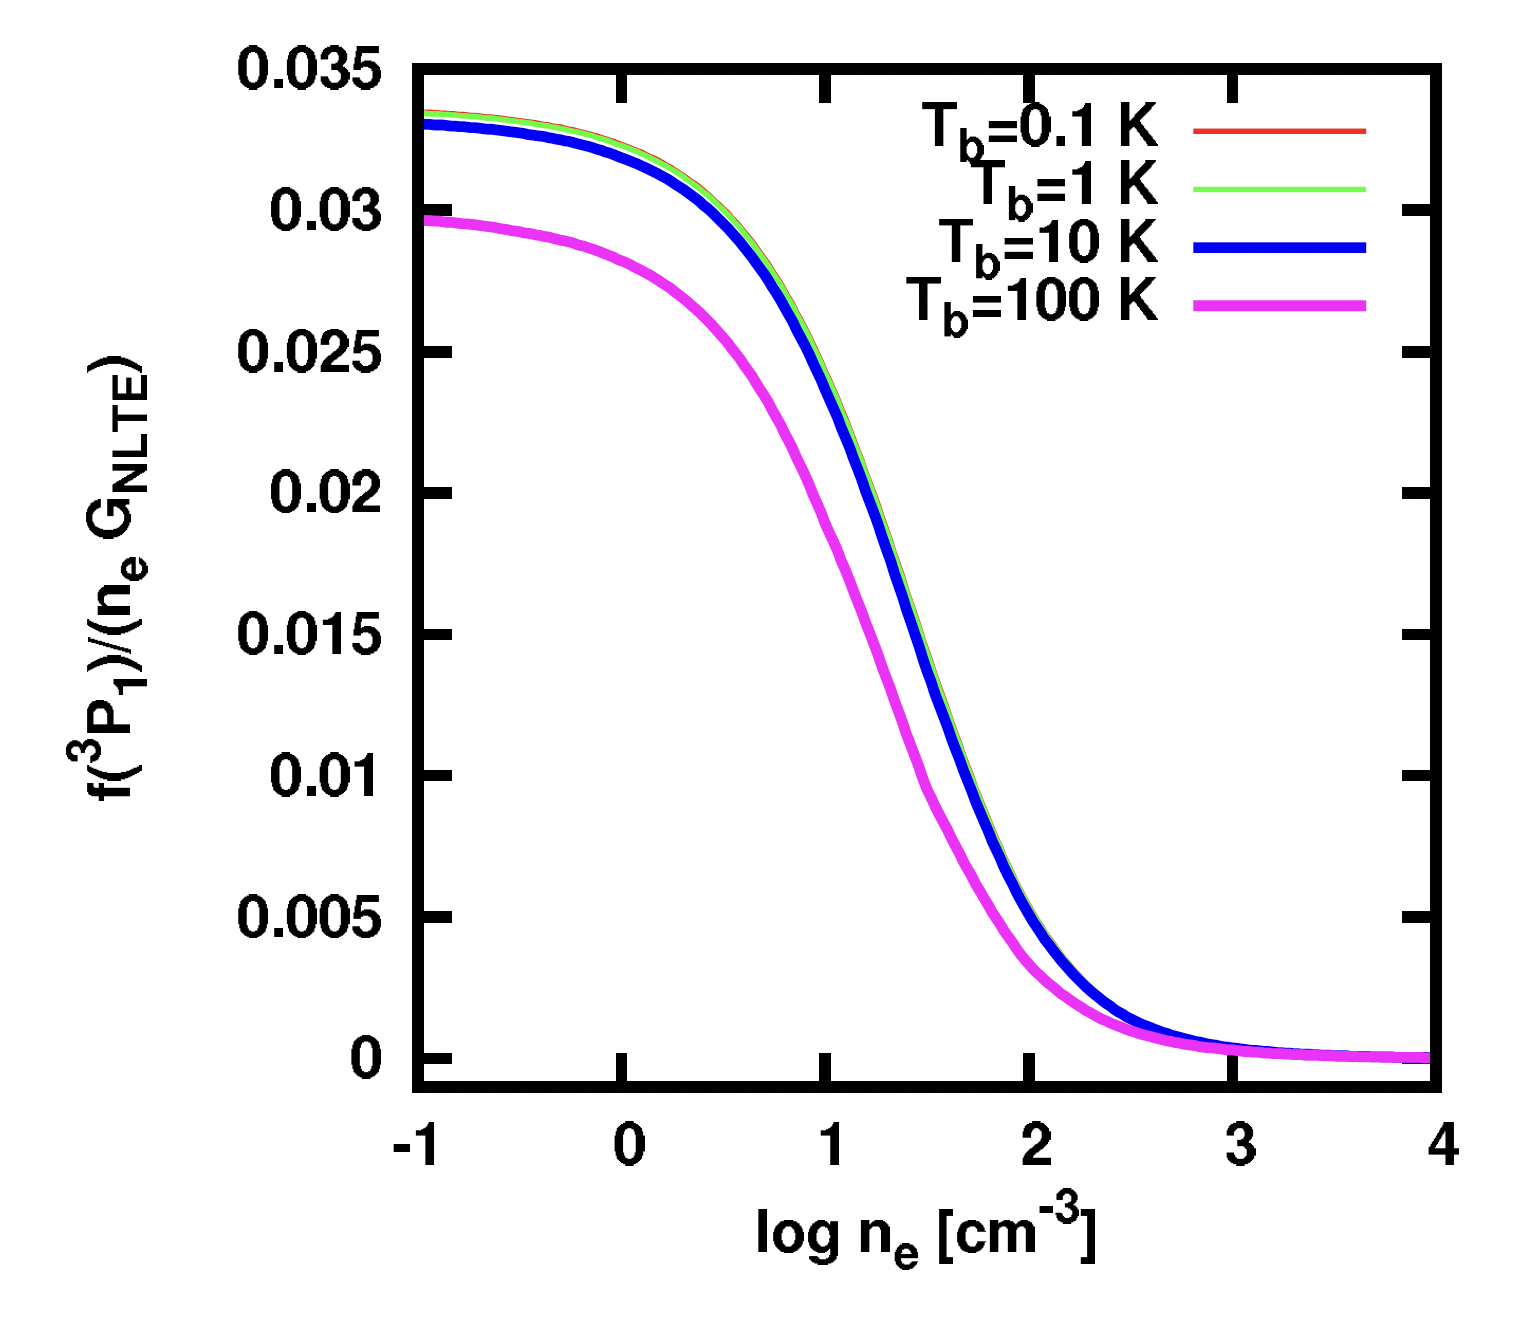
\includegraphics[width=0.4\textwidth]{figs/4/curve.png}
    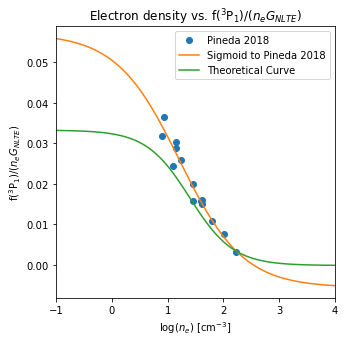
\includegraphics[width=0.4\textwidth]{figs/4/calculated_curve.png}
    \caption{The dependence of the [NII] 205 $\mu$m ratio on delectron density for a set of continuum brightness temperatures \cite{pineda2018}.}
    \label{fig:ne_vs_tc}
\end{figure}

With this sigmoid, we can now calculate the electron density for the Carina Nebula assuming our continuum brightness is between 0.1 and 10 K.
To prepare both spectral cubes we spectrally and spatially reproject the [NII] 205 $\mu$m and the Hydrogen RRL data to the same grid.
We then convolve the [NII] 205 $\mu$m data with the beam of the RRL data. 
Finally, we calculate the integrated intensities of both lines for the following locations.

\begin{table}[h!]
    \centering
    \begin{tabular}{|c|c|c|}
        \hline
        Location & $v_{min}$ km/s & $v_{max}$ km/s \\
        \hline
        Keyhole Nebula & -40 & -20 \\
        Carina Extended & -20 & 20 \\
        \hline
    \end{tabular}
    \caption{The spectral slabs of Carina Nebula used to calculate the electron density.}
    \label{tab:carina}
\end{table}

The resultant electron density map is shown in Figure \ref{fig:ne_map_keyhole} and \ref{fig:ne_map_carina}.

\begin{figure}[h]
    \centering
    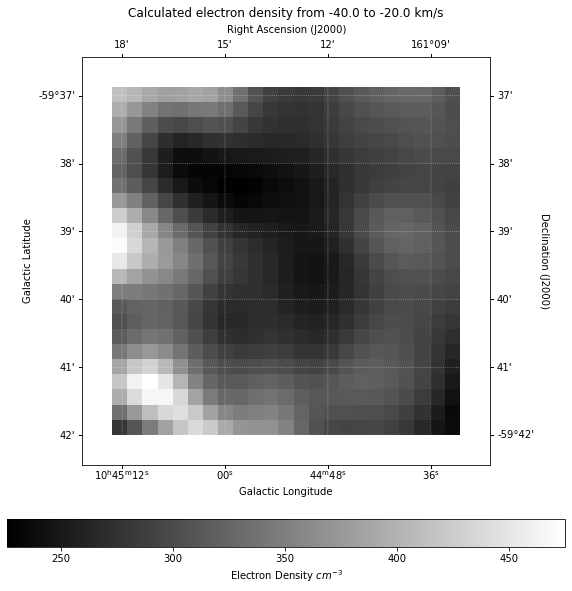
\includegraphics[width=\textwidth]{figs/4/ne_map_keyhole.png}
    \caption{The electron density map of the Keyhole Nebula.}
    \label{fig:ne_map_keyhole}
\end{figure}

\begin{figure}[h]
    \centering
    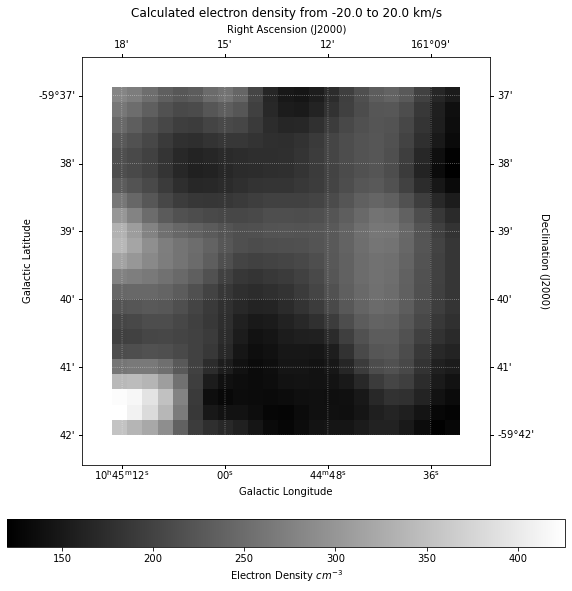
\includegraphics[width=\textwidth]{figs/4/ne_map_carina.png}
    \caption{The electron density map of Carina Extended.}
    \label{fig:ne_map_carina}
\end{figure}

